\documentclass[pt]{standalone}
\usepackage{amsmath}
\usepackage{graphicx}
\usepackage[pdf]{pstricks}
\usepackage{pgfplots}
\pgfplotsset{compat=newest}
\usepgfplotslibrary{fillbetween}
%% the following commands are needed for some matlab2tikz features
\usetikzlibrary{plotmarks}
\usetikzlibrary{arrows.meta}
\usepgfplotslibrary{patchplots}
\usetikzlibrary{decorations.text}
\usetikzlibrary{shapes.multipart}
%\usetikzlibrary{external}
%\tikzexternalize % activate!

\begin{document}
\begin{tikzpicture}
\node[inner sep=0pt] (BetaPlot) at (0,0)
{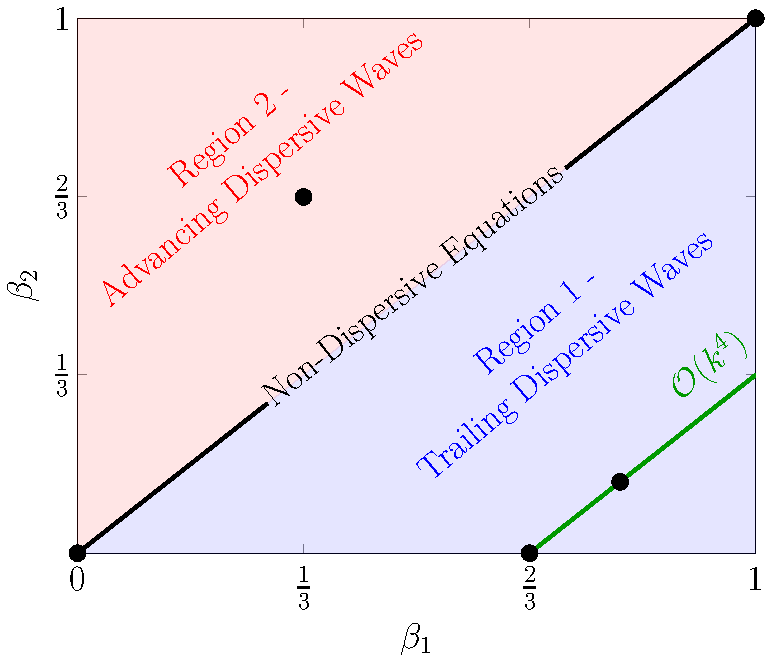
\includegraphics[width=0.45\textwidth]{BetaPlotAllWithExamples.pdf}};
\node[inner sep=0pt] (SWWE) at (-4.5,-4)
{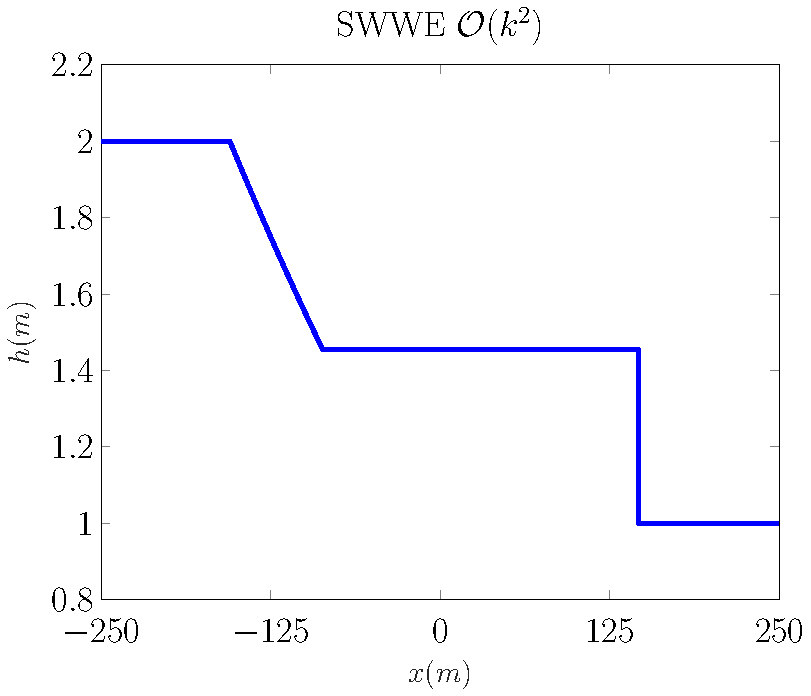
\includegraphics[width=0.3\textwidth]{hEx03.pdf}};

\node[inner sep=0pt] at (-4.5,-5.8){\scriptsize (d)};
\draw[->,dotted,thick,opacity=0.5] (-2.2,-1.6) -- (-3.8,-2.5) ;
\node[inner sep=0pt] (SGN) at (4.5,-4)
{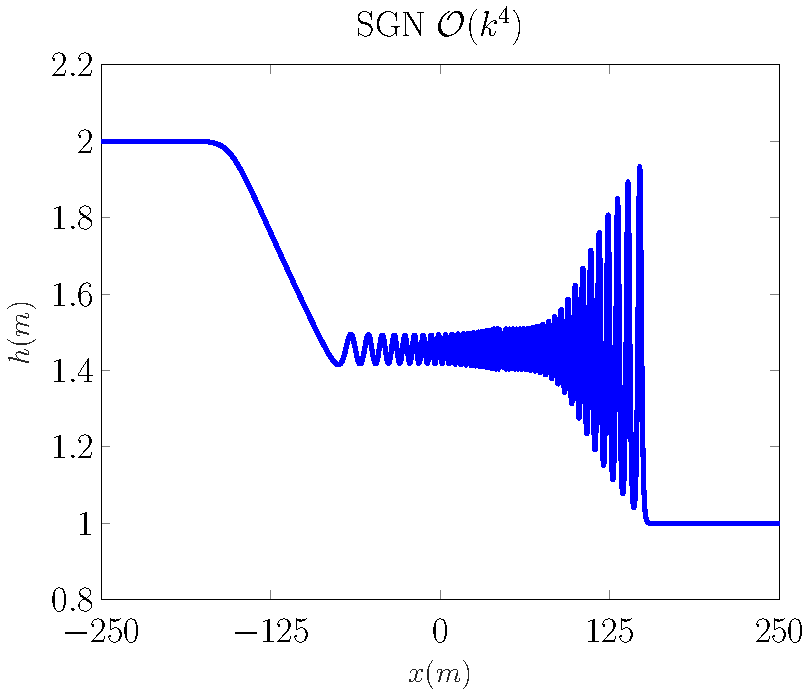
\includegraphics[width=0.3\textwidth]{hEx00.pdf}};
\node[inner sep=0pt] at (4.5,-5.8){\scriptsize (e)};
\draw[->,dotted,thick,opacity=0.5] (1,-1.6) -- (4.2,-2.5) ;

\node[inner sep=0pt] ((iSGN) at (4.5,0)
{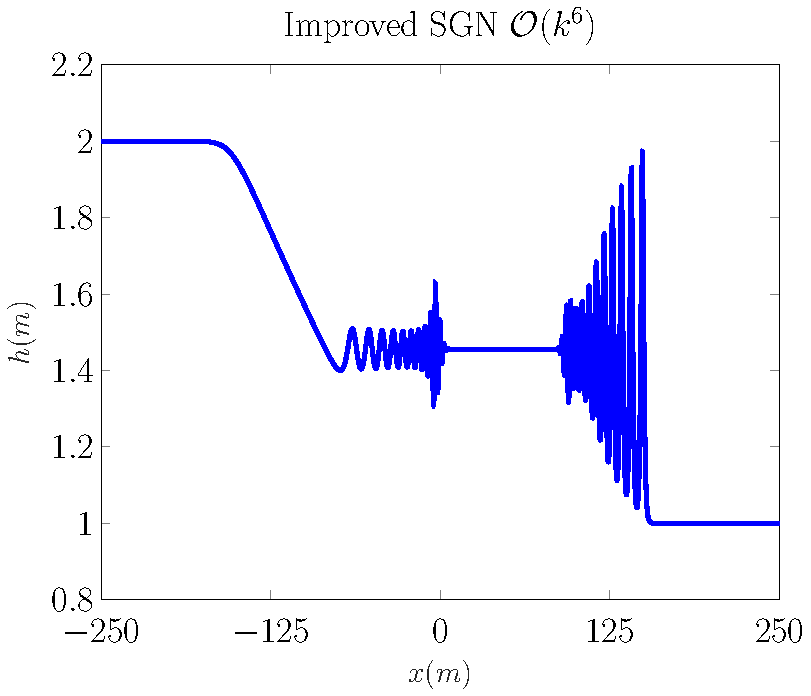
\includegraphics[width=0.3\textwidth]{hEx01.pdf}};
\node[inner sep=0pt] at (4.5,-1.8){\scriptsize(c)};
\draw[->,dotted,thick,opacity=0.5] (1.7,-1) -- (4.3,1.3) ;

\node[inner sep=0pt] ((rSWWE) at (4.5,4)
{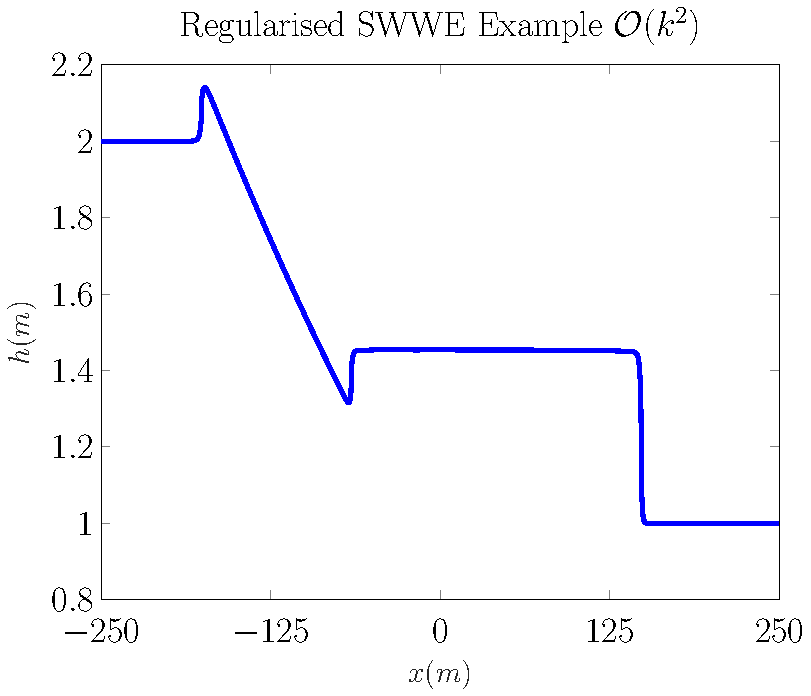
\includegraphics[width=0.3\textwidth]{hEx02.pdf}};
\node[inner sep=0pt] at (4.5,2.2){\scriptsize(b)};
\draw[->,dotted,thick,opacity=0.5] (2.6,2.2) -- (4.3,5.3) ;

\node[inner sep=0pt] ((Reg2) at (-4.5,4)
{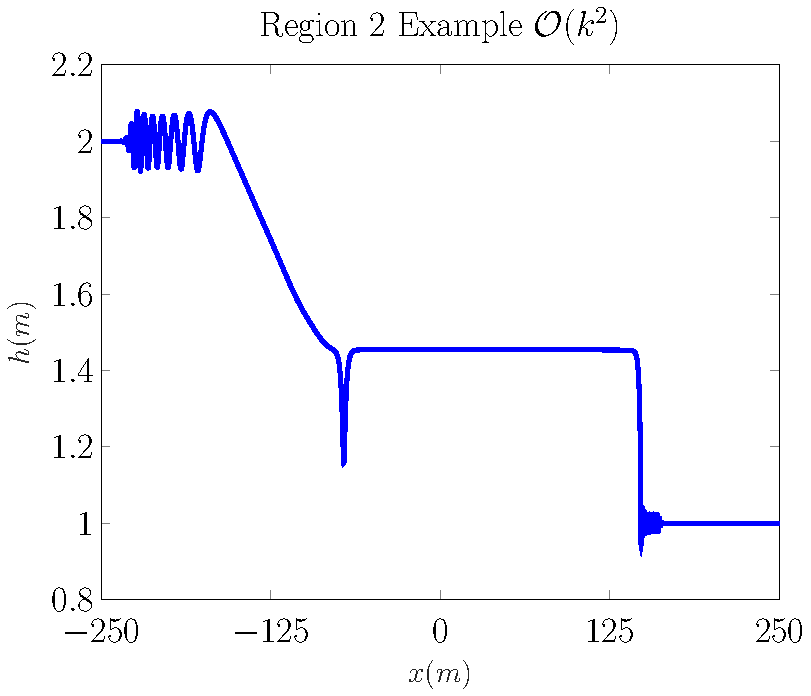
\includegraphics[width=0.3\textwidth]{hEx04.pdf}};
\node[inner sep=0pt] at (-4.5,2.2){\scriptsize (a)};
\draw[->,dotted,thick,opacity=0.5] (-0.6,1) -- (-4.3,5.3) ;



%\node[inner sep=0pt] (rSWWE) at (4,3.5)
%{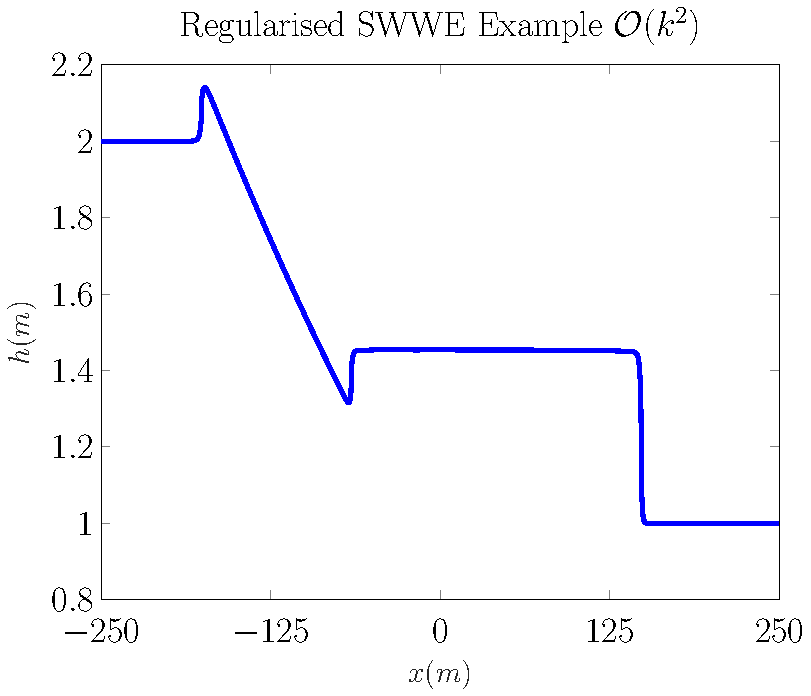
\includegraphics[width=0.33\textwidth]{hEx02.pdf}};
%\node[inner sep=0pt] (iSGN) at (4,0)
%{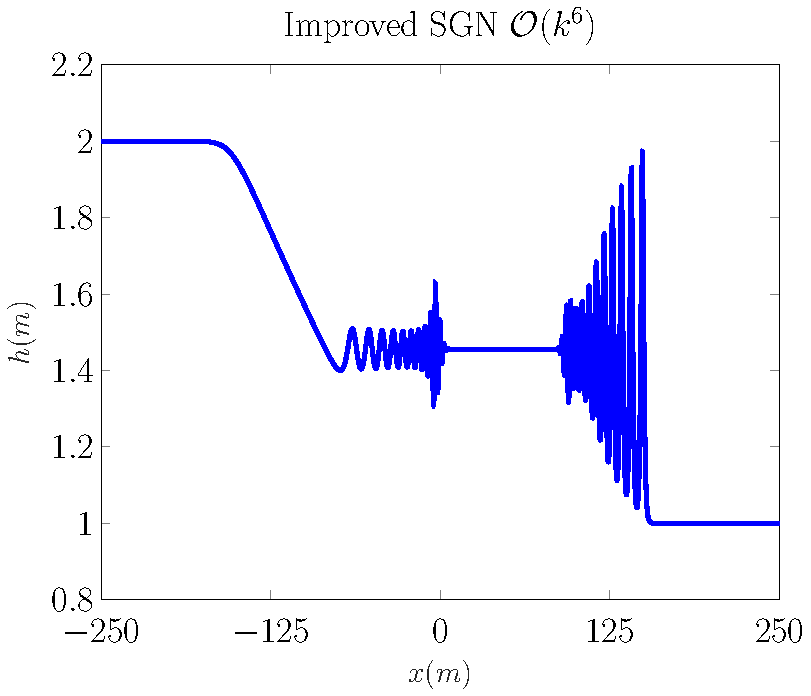
\includegraphics[width=0.33\textwidth]{hEx01.pdf}};
%\node[inner sep=0pt] (Reg2) at (-4,3.5)
%{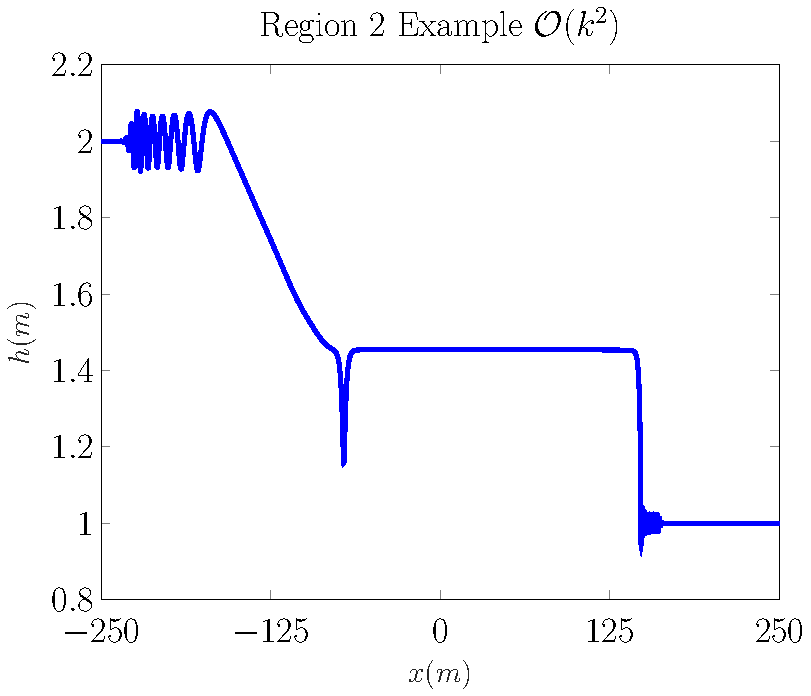
\includegraphics[width=0.33\textwidth]{hEx04.pdf}};
%\draw[->,dotted,thick,opacity=0.5] (-1.7,-1.23) -- (-3.5,-2) ;
%\draw[->,dotted,thick,opacity=0.5] (0.7,-1.25) -- (0.2,-1.95) ;
%\draw[->,dotted,thick,opacity=0.5] (1.3,-0.8) -- (3,-0.8) ;
%
%\draw[->,dotted,thick,opacity=0.5] (2,1.7) -- (3,2.5) ;
%\draw[->,dotted,thick,opacity=0.5] (-0.42,0.7) -- (-4,2.5) ;
\end{tikzpicture}
\end{document}